\documentclass[11pt,a4paper]{article}
\usepackage[utf8x]{inputenc}
\usepackage{graphicx}
\usepackage{esdiff}
\usepackage[english]{babel}
\usepackage{color}
\usepackage{float}
\usepackage{epstopdf}
\usepackage{afterpage}
\usepackage{caption}
\usepackage{subcaption}
\captionsetup[table]{oneside , margin = {2cm, 0cm},
	justification=RaggedRight, singlelinecheck = false }
\usepackage{subcaption}
\usepackage{mathtools}
\usepackage{multicol}
\usepackage{algorithm2e}
\usepackage{titling}
\usepackage{amsmath}
\usepackage[colorlinks=true]{hyperref} % the option is there to remove the square around links which is what I don't like.
\usepackage{comment}
\usepackage{perpage} 
\MakePerPage{footnote} % Reset the footnote counter perpage. may require to run latex twice.

\usepackage[margin=2cm]{geometry} % This is here to fit more text into the page.

%\setcounter{secnumdepth}{1}  % This removes the numbering from the subsections.
% If you want the numbering of the subsection level just remove this line
\usepackage{titling}
\newcommand{\subtitle}[1]{%
	\posttitle{%
		\par\end{center}
	\begin{center}\large#1\end{center}
	\vskip0.5em}%
}



\setlength{\parindent}{0pt} % No indentation for paragraphs. Because that is just old.
\setlength{\parskip}{\baselineskip} % Instead use vertical paragraph spacing.

\fontencoding{T1} % the better font encoding.
\title{\textsc{Assignment Optimal Control Problem}}
\subtitle{\textsc{Advanced Optimization-based Robot Control Final Project}}	
\date{11/06/2020}
\author{Jacopo Antonini, Giorgio Checola} 
%\setmainfont{Helvetical} % Setting the main font here. But I like the default font alot so this is commented out.
\makeatletter
\def\@maketitle{
	\graphicspath{ {./images/} }
	
\includegraphics[width=100mm]{unitn-logo}
	\begin{center}
		
	
	\item {\Huge \bfseries \@title } 
	\item { \Large Advanced optimiza}
	\item {\Large  \@author}  
	\item \@date 
	
	
	

	\item matr. 197729
	\item Department of Industrial Engineering
	\item {Università degli studi di Trento}
	\\

	\end{center}
}
\makeatother
\begin{document}
	
	\graphicspath{ {./images/} }
	\maketitle
	\thispagestyle{empty}
	\newpage
	\thispagestyle{empty}
	\mbox{}
	\newpage
	
	
	
	\section*{Abstract}
		The metal-oxide semiconductor or MOS is a type of transistor which consists of a doped silicon substrate, two heavily doped regions called drain and source, an oxide layer deposited on top and between drain and source. In figure \ref*{fig:mosfet} is shown the layout of the structure.
			\begin{figure}[h]
				\centering
				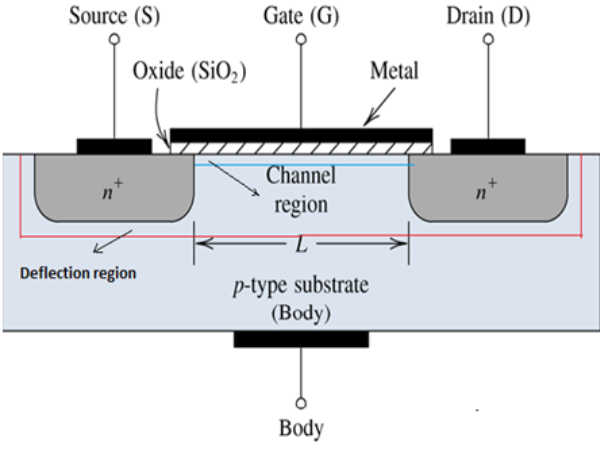
\includegraphics[width=100mm]{mosfet}
				\caption{Basic structure of a MOSFET device.}
				\label{fig:mosfet}
			\end{figure}
		\begin{enumerate}
			\item asas
		\end{enumerate}	
	\section{Introduction}
		This project is done starting by the structure shown in figure \ref*{fig:struttura}. The substrate is obtained by an epitaxial layer on top of a silicon bulk. The drain and the source are obtained doping two regions of the substrate with a $n^+$ Gaussian profile with junction depth \(x_j\). All the geometrical parameters are listed in the Table \ref*{geom}.
		\begin{figure}
			\centering
			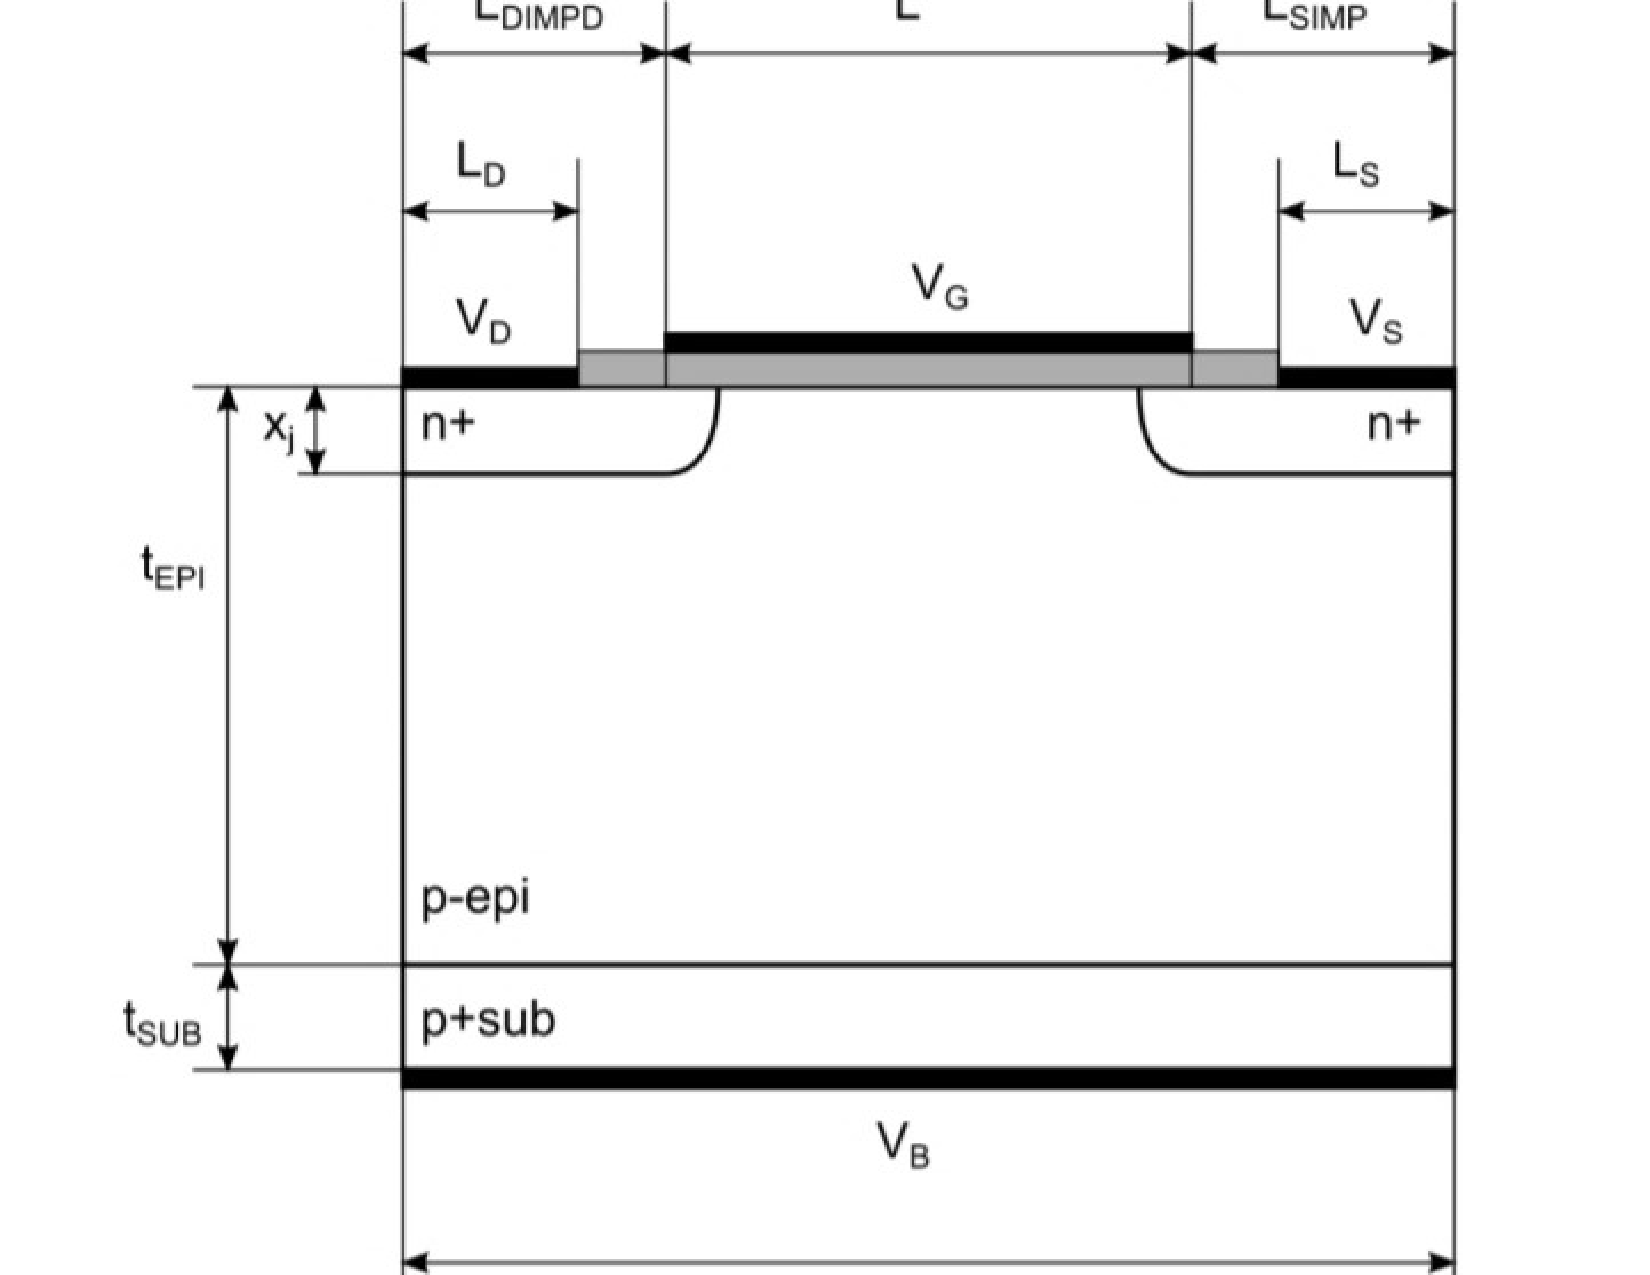
\includegraphics[width=100mm]{struttura}
			\caption{Structure of the NPN MOSFET used for simulation.}
			\label{fig:struttura}
		\end{figure}	
		\begin{table}[h]
			\captionsetup{oneside,margin={2cm,0cm},justification = RaggedRight}
			\caption{Geometrical Parameters}
			\centering
			\begin{tabular}[H]{|| c | c | c | c ||}
				\hline
				Parameter & $[\mu m]$ & Parameter & $[\mu m]$ \\ [0.5ex] 
				\hline\hline
				$W_{DEV}$ & 4 & $t_{EPI}$& 3 \\
				\hline
				$t_{SUB}$ & 1 & $L$        & 3 \\
				\hline
				$L_{DIMP}$ & 0.5 & $L_{SIMP}$ & 0.5\\
				\hline
				$L_{D}$ & 0.3 & $L_{S}$& 0.3\\
				\hline
				$t_{ox}$ & $30 \cdot 10^{-3} $ &- &-\\
				\hline
			\end{tabular}
			\label{geom}
		\end{table}
	\section{Structure}
	The structure obtained is shown in figure \ref*{fig:doping}, in which we can see that there is a constant profile in the epitaxial region and in the remaining substrate, with concentration $10^{16} \frac{at.B}{cm^{3}}$ and $10^{19} \frac{at.B}{cm^3}$ respectively. It can also be noticed that the doping profile in the source and drain regions is Gaussian. The specification of the problem imposed the junction depth $x_j$ to be $0.5 \mu m$, the characteristic length $L_{c}$ to be $0.1 \mu m$ and the peak donor concentration $C_p$ is $10^{19} \frac{at.P}{cm^3}$. The location of the peak concentration in the profile is not specified, and if we assume it to be at the surface of the device the two situations shown in figure \ref*{gauss1} and \ref*{gauss2} arise. So clearly the position of the maximum should be elsewhere and the mathematical expression becomes: \[ C(x) = C_p \cdot e^{-(\frac{x-x_p}{L_{c}})^2},\] where $x_p = 0.24 \mu m$. The final Gaussian profile is shown in figure \ref*{gauss4}. 
	The mesh used for the simulation is represented in figure \ref*{meshing} and a detail about a critical region in figure \ref*{meshingdetail}.
	
		\begin{figure}
			\centering
			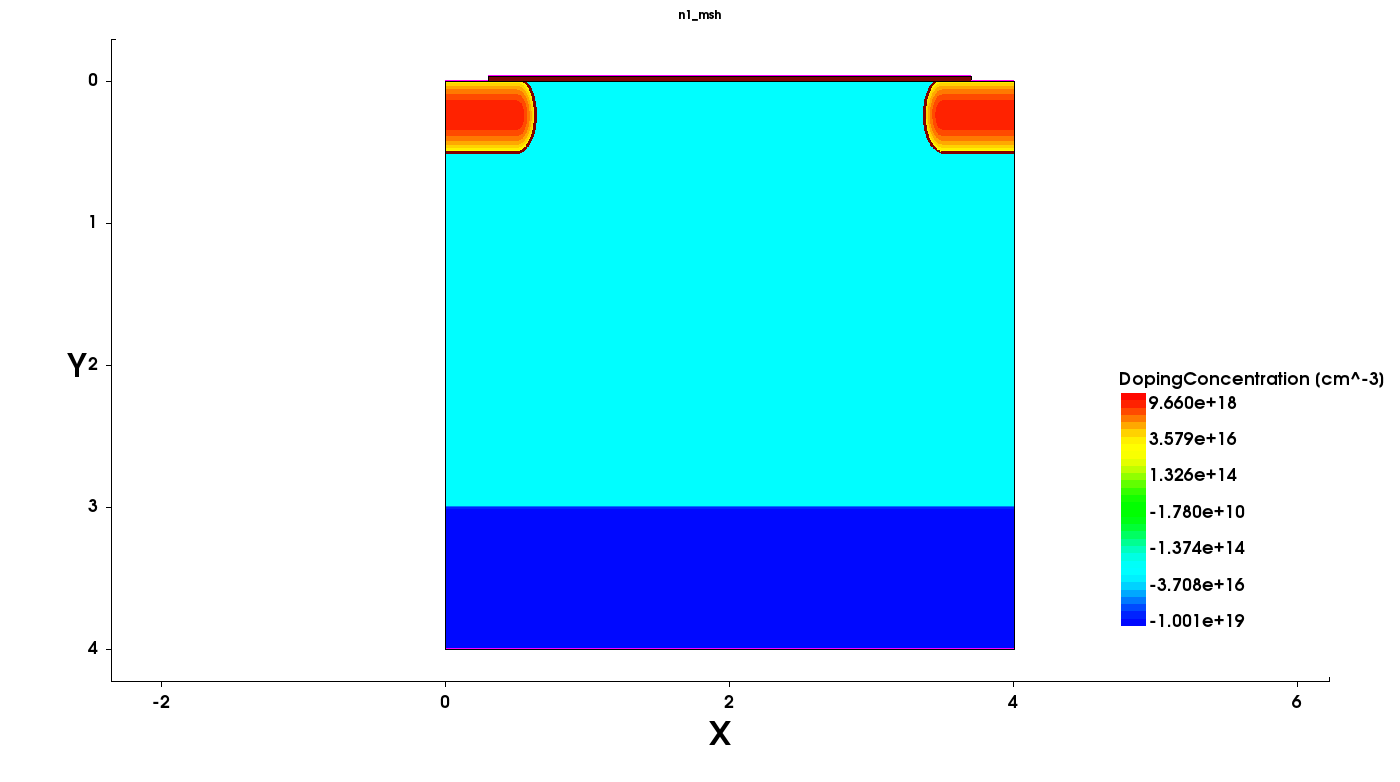
\includegraphics[width=100mm]{doping1}
			\caption{Doping profile of the MOSFET device.}
			\label{fig:doping}
		\end{figure}
		\begin{figure}
			\centering
			\begin{subfigure}[b]{0.45\textwidth}
				\centering
				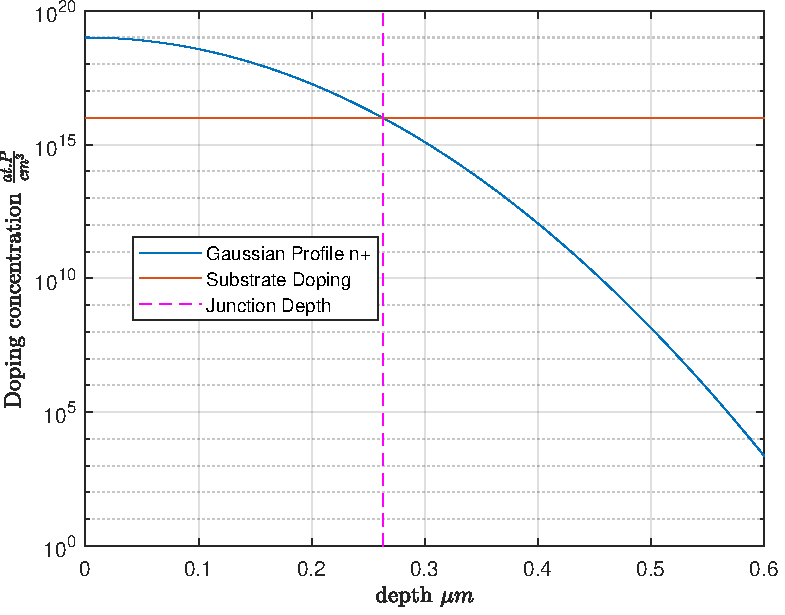
\includegraphics[width=\textwidth]{gauss1.pdf}
				\caption{Doping profile if peak is imposed.}
				\label{gauss1}
			\end{subfigure}
			\hfill
			\begin{subfigure}[b]{0.45\textwidth}
				\centering
				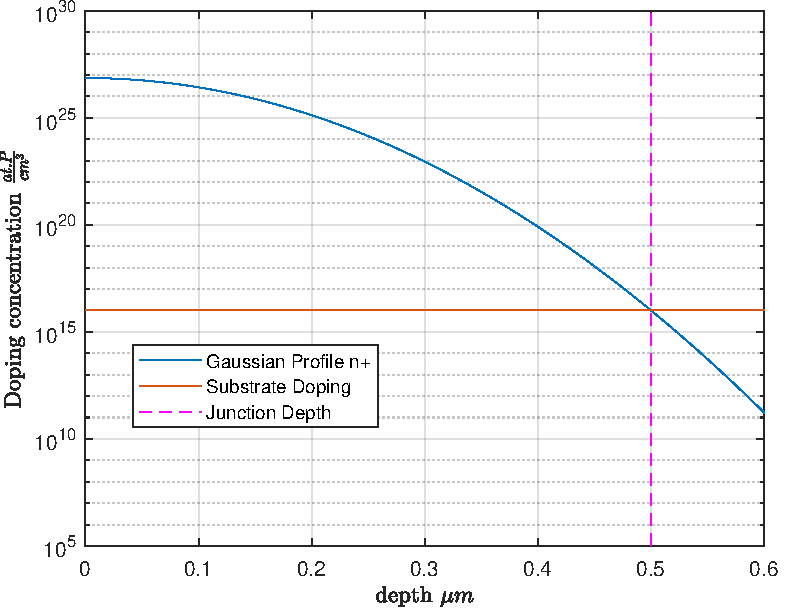
\includegraphics[width=\textwidth]{gauss2.pdf}
				\caption{Doping profile if junction depth is imposed.}
				\label{gauss2}
			\end{subfigure}
			\caption{Gaussian profile with peak on the surface.}
		\end{figure}
		\begin{figure}
			\centering
			\includegraphics[width=80mm]{gauss4}
			\caption{Final Gaussian profile}
			\label{gauss4}
		\end{figure}
		\begin{figure}
			\centering
			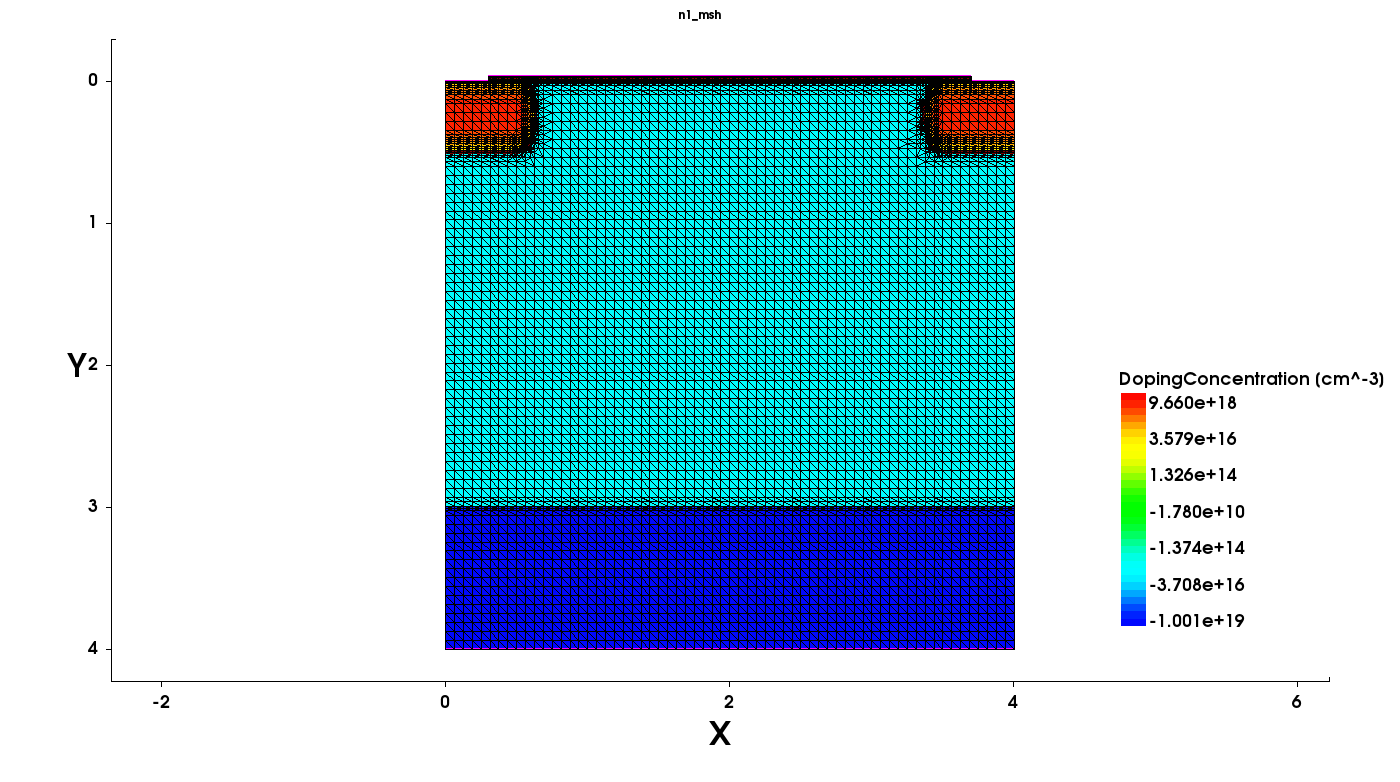
\includegraphics[width=100mm]{meshing1}
			\caption{Mesh}
			\label{meshing}
		\end{figure}
		\begin{figure}
			\centering
			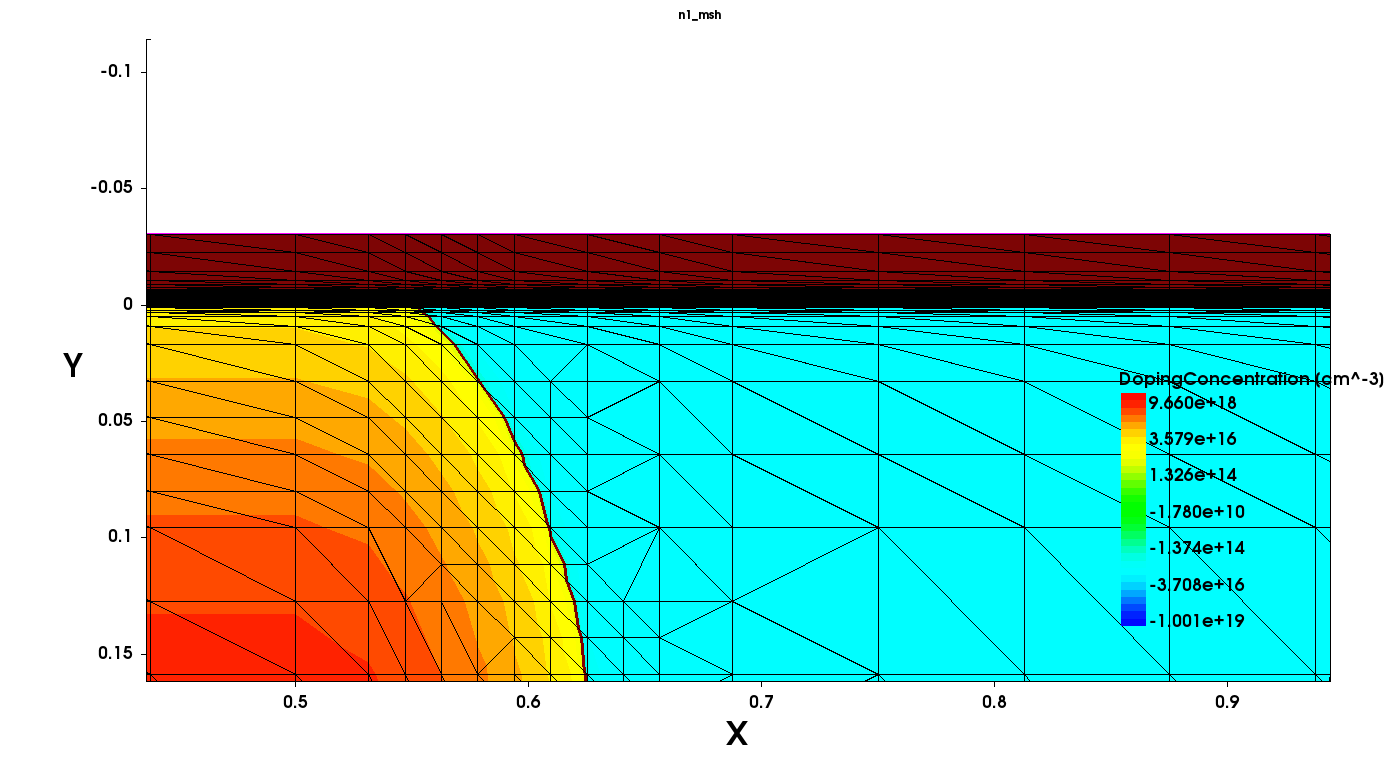
\includegraphics[width=80mm]{meshing_detail}
			\caption{Detail of the mesh}
			\label{meshingdetail}
		\end{figure}
		
	%gaussian profile and calculations
	%simulation domain, meshing
	\section{Simulations}
	%equilibrium state
	\subsection{Equilibrium}
	The first simulation done, whose result is in figure \ref*{equilibrium}, is about the equilibrium state, where in \ref*{elecpotential} the electrostatic potential is shown and in figure \ref*{currents} the total current due to the normal movement of the charge carriers. They are calculated imposing all the electrodes to 0V.
		\begin{figure}
			\centering
			\begin{subfigure}[b]{0.45\textwidth}
				\centering
				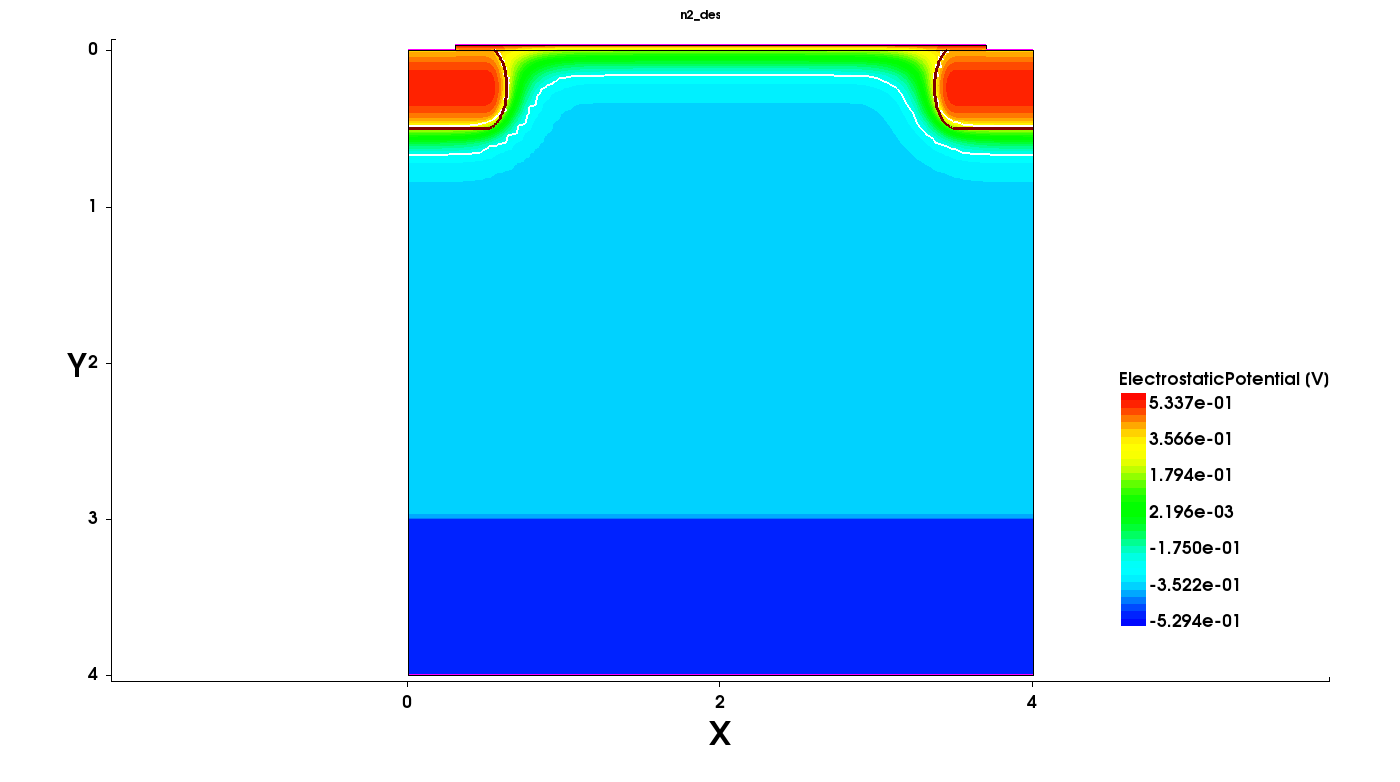
\includegraphics[width=\textwidth]{electrostatic_potential11.png}
				\caption{Electrostatic potential.}
				\label{elecpotential}
			\end{subfigure}
			\hfill
			\begin{subfigure}[b]{0.45\textwidth}
				\centering
				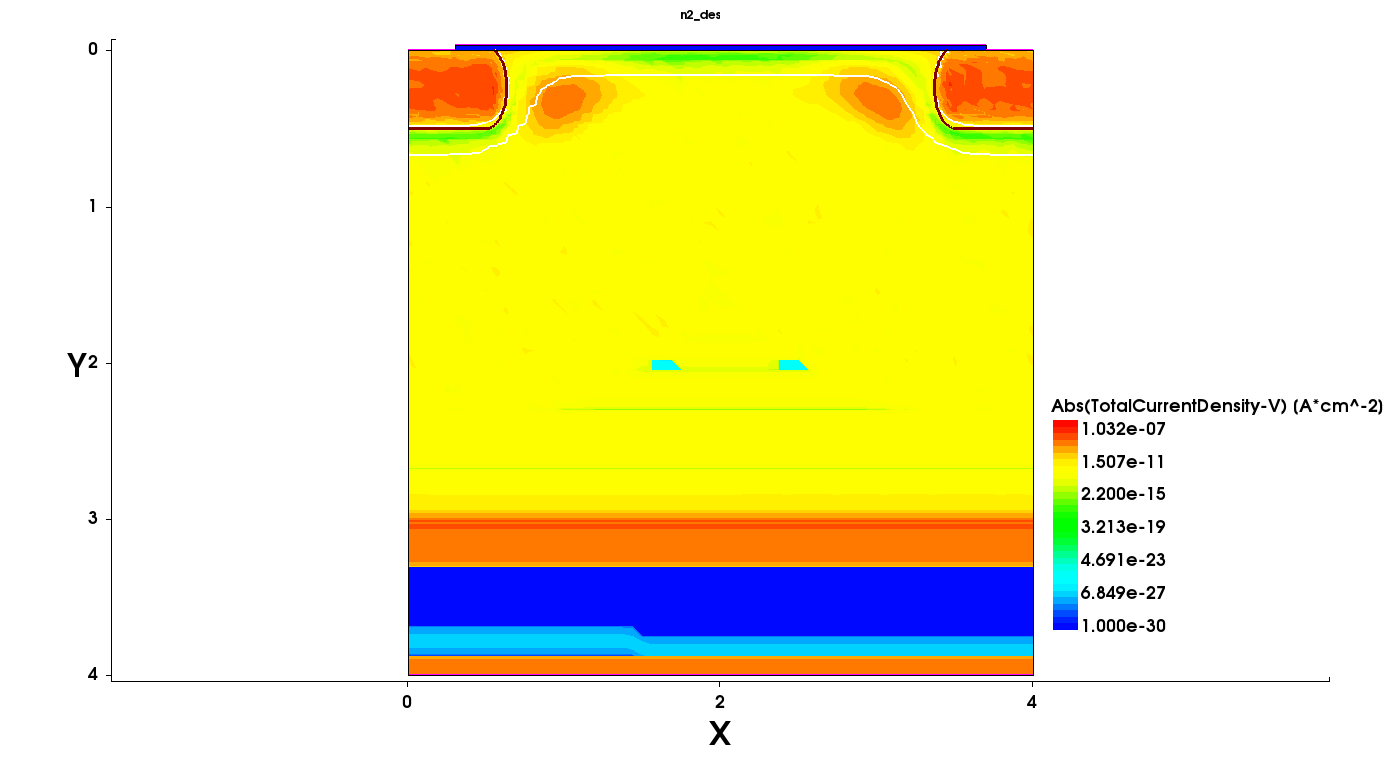
\includegraphics[width=\textwidth]{currents.png}
				\caption{Absolute current density.}
				\label{currents}
			\end{subfigure}
			\caption{Simulation at equilibrium condition.}
			\label{equilibrium}
		\end{figure}
	\subsection{Transfer Characteristic}
	The second simulation consists in finding the transfer characteristic, which is the relation that express the dependency of the drain current \(I_D\) with respect to the gate and threshold voltages. The formula is the following: 
	\begin{equation} \label{trans_char}
	I_D = \frac{K_n}{2}(V_{GS}-V_{TH})^2.
	\end{equation}
	This relation holds when the MOSFET is in saturation, namely when $V_{DS} \geq V_{GS}-V_{TH}$. The simulation has been done by sweeping the gate voltage from 0 to a 5V because, since the bias imposed by the problem is $V_{DS} = 5V$ and the analytical calculation give $V_{TH} \approx 0.4V$, going further with the $V_{GS}$ value could make the MOSFET be in the quasi-linear region where the output characteristic is 
	\begin{equation} \label{output_char}
	I_D = K_n \left[\left(V_{GS}-V_{TH}\right)V_{DS}-\frac{{V_{DS}}^2}{2}\right].
	\end{equation}
	Also this formula could be used to identify $K_n$ and $V_{TH}$ since we know the value of $V_{DS}$, but finding a single function that describe these two behaviours (quasi-linear and saturated) can be too difficult. Anyway, the identification is done by linear interpolation of the square of the transfer characteristic: 
	\begin{equation} \label{sqr_trans_char}
		\sqrt{I_D} = \sqrt{\frac{K_n}{2}}(V_{GS}-V_{TH}).
	\end{equation} 
	Figure \ref*{identification} and table \ref*{identification_results} show the processing done and the results obtained.
	\begin{figure}
		\centering
		\begin{subfigure}[b]{0.45\textwidth}
			\centering
			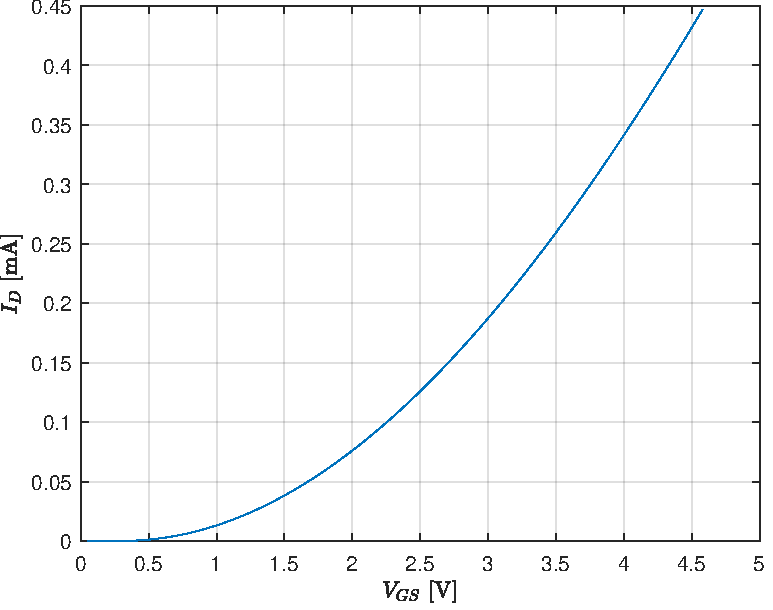
\includegraphics[width=\textwidth]{parabola}
			\caption{Simulated transfer characteristic.}
			\label{parabola}
		\end{subfigure}
		\hfill
		\begin{subfigure}[b]{0.45\textwidth}
			\centering
			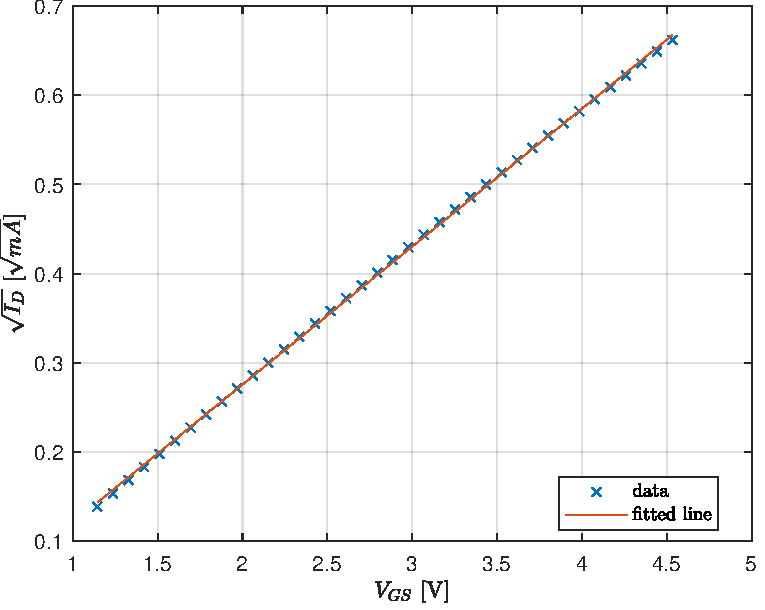
\includegraphics[width=\textwidth]{sqrt_fit}
			\caption{Square root of drain current.}
			\label{sqrt_fit}
		\end{subfigure}
		\caption{Identification of Threshold and Current Gain.}
		\label{identification}
	\end{figure}
	\begin{table}
		\captionsetup{oneside,margin={2cm,0cm},justification = RaggedRight}
		\caption{Results of the identification}
		\centering
		\begin{tabular}[H]{|| c | c | c ||}
			\hline
			Parameter & Value & Measure Unit \\ [0.5ex] 
			\hline\hline
			$V_{TH}$ & 0.22 & $V$\\
			\hline
			$\beta$ & $4.78\cdot 10^{-2}$ & $\frac{mA}{V^2}$\\
			\hline			
		\end{tabular}
		\label{identification_results}
	\end{table}
	%%%%%%%%%%%%%%%%%%%%%%%%%%%%%%%%%%%%%%IDENTIFICAZIONEEEEEEEEEEEEEEEEEEEEE
	\subsection{Small Signal Output Resistance}
	In order to know the small signal output resistance, the first simulation to do is a sweep from 0V to 5V of the $V_{DS}$, biased at $V_{GS} = 2,3,4V$. A small signal is an AC voltage that is overlapped to a DC one whose amplitude is quite higher than the other one. In the case of the drain-source voltage it can be called $v_{DS} = V_{DS} + v_{ds}$. The result, at a certain gate voltage, will be $i_D = I_D+i_d$, so a small AC current plus a DC bias. This kind of result is due to the superposition effect, that holds for linear devices. A MOSFET transistor is not a linear device with respect to $v_{DS}$, especially in the quasi-linear region, expressed by equation \ref*{output_char}, where the dependency is quadratic. But if the channel modulation effect is considered, the equation \ref*{trans_char} of saturation condition becomes:
	\begin{equation} \label{channel_mod}
		 i_D = \frac{K_n}{2}(v_{GS}-V_{TH})^2(1+\lambda v_{DS}),
	\end{equation}
	that is linear in $v_{DS}$. Since $i_D$ is a function of $v_{DS}$ it can be expressed as $i_{D}(V_{DS}+v_{ds}) = I_D + i_d $ and can be seen as a Taylor expansion of the first order: 
	\begin{equation} \label{taylor}
	f(x) = f(X+\Delta x) = f(X)+ \frac{df(x)}{dx} \Bigr\rvert_{x = X} \Delta x.
	\end{equation}
	Using this reasoning we can understand that $i_d = \frac{di_D}{dv_{DS}}\Bigr\rvert_{v_{DS} = V_{DS}}v_{ds} = \frac{1}{R_{ss}}v_{ds}$, so the small signal output resistance is just the inverse of the slope of the I-V curve evaluated at $V_{DS}$. Since $V_{TH} > 0$, the saturation condition for $V_{DS} = 4$ is valid for each of the $V_{GS}$ that we are going to use. Figure \ref*{outputcurve} shows the results of the simulation and table \ref*{resistances} reports the small signal output resistances for the three values of $V_{GS}$.
	\begin{figure}
		\centering
		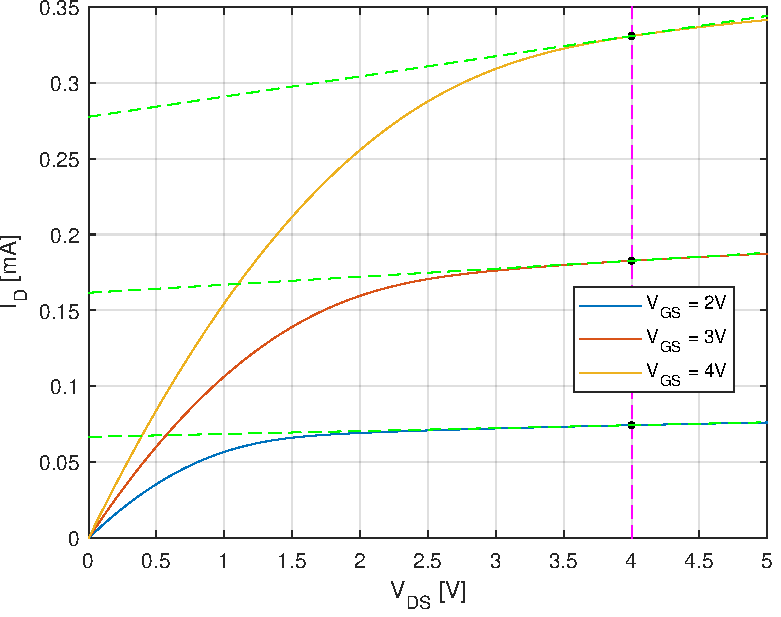
\includegraphics[width=100mm]{output_curves}
		\caption{Output characteristic}
		\label{outputcurve}
	\end{figure}
	\begin{table}
		\captionsetup{oneside,margin={2cm,0cm},justification = RaggedRight}
		\caption{Small signal output resistances}
		\centering
		\begin{tabular}[H]{|| c | c | c | c ||}
			\hline
			Gate Bias & $[V]$ & Resistance & $[k\Omega]$ \\ [0.5ex] 
			\hline\hline
			$V_{GS2}$ & 2 & $R_{ss2}$& 520\\
			\hline
			$V_{GS3}$ & 3 & $R_{ss3}$& 190\\
			\hline
			$V_{GS4}$ & 4 & $R_{ss4}$& 75\\
			\hline			
		\end{tabular}
		\label{resistances}
	\end{table}
	\subsection{Gate Capacitance}
	The metal-oxide structure of the gate region works exactly like a capacitor, because is like two conductive plates and a dielectric material in between. Since the area is much larger than the thickness of the oxide, the general formula for the capacitance holds: 
	\begin{equation}\label{cox}
		C_{ox} = \frac{\epsilon_{ox}}{t_{ox}}. 
	\end{equation} In addition to this behaviour, the is another capacitor cascaded to the previous one, whose dielectric material is the silicon itself and the plates are represented by the charges of the space-charge-region. Actually they are not real conductive plate, but since there are two opposite charge distributions around a dielectric material, a capacitive behaviour is observed. Therefore, the thickness of the silicon dielectric is represented by the space-charge-region width. This quantity is not fixed, like the oxide thickness as a technological parameter, but depends on the gate voltage, increasing from zero to a maximum as the gate bias reaches the threshold voltage.
	\begin{equation}\label{scr}
		w[\Psi_s(V_{GS})] = \sqrt{\frac{2\epsilon_s}{qN_A}\left(\Psi_s(V_{GS})\right)}.
	\end{equation}  
	The maximum space-charge-region is reached when $V_{GS} = V_{TH} \Rightarrow \Psi_s = 2\varphi_F$ and is equal to:
	\begin{equation}\label{scr}
	w_m = \sqrt{\frac{2\epsilon_s}{qN_A}(2\varphi_F)}.
	\end{equation} 
	So, given that the relation for planar capacitors holds:
	\begin{equation}
		C_{si} = \frac{\epsilon_s}{w[\Psi_s(V_{GS})]} = \frac{\epsilon_s}{\sqrt{\frac{2\epsilon_s}{qN_A}\left(\Psi_s(V_{GS})\right)}} \quad for \quad  V_{GS}<V_{TH}
	\end{equation} and the minimum value is:
	\begin{equation} \label{cmin}
		C_{min} = \frac{\epsilon_s}{w_m} = \frac{\epsilon_s}{\sqrt{\frac{2\epsilon_s}{qN_A}\left(2\varphi_F\right)}} \quad for \quad  V_{GS}\geq V_{TH}.
	\end{equation}
	The overall value of the capacitance is obtained by calculating the series of the two capacitors:
	\begin{equation}
		C_{tot} = \frac{C_{ox} \cdot C_{si}}{C_{ox}+C_{si}}.
	\end{equation} 
	The simulated result of capacitance as a function of the gate voltage is shown in figure \ref*{capacitance1}.
	\begin{figure}
		\centering
		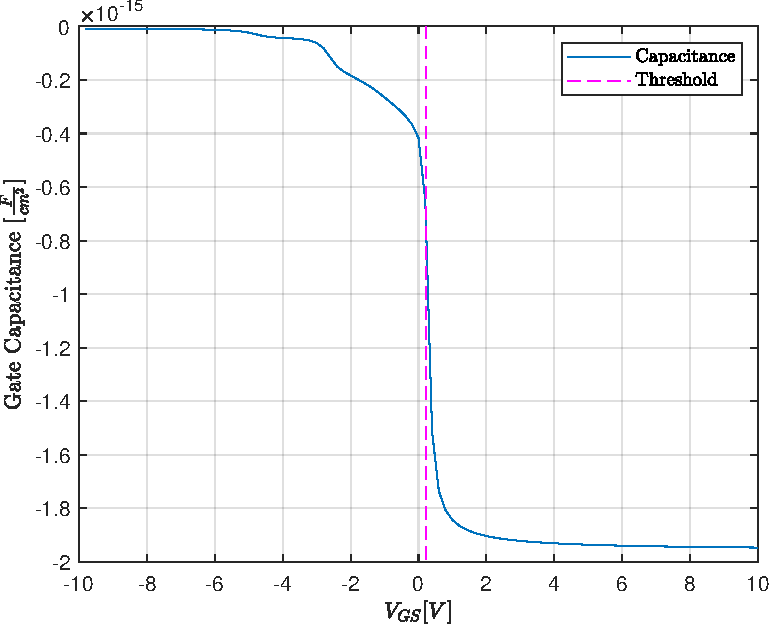
\includegraphics[width=100mm]{capacitance1}
		\caption{Gate capacitance as a function of $V_{GS}$}
		\label{capacitance1}
	\end{figure}
	\section{Threshold Adjustment}
	An operation that can be done on a MOSFET transistor to adjust the value of the threshold voltage is an ion implantation. Equations from \ref*{idealthreshold} to \ref*{thresholdadjust}, quantify how much the threshold can be shifted related to the charge density deposited by the ion implantation process. $\Phi_{ms}$ is the metal-semiconductor workfunction difference, $Q_{eq}$ is the equivalent charge density of the oxide due to ionic contamination.
	\begin{equation}\label{idealthreshold}
		V_{TH-IDEAL} = \frac{\sqrt{2\epsilon_s q N_A\left(2\varphi_F\right)}}{\epsilon_{ox}/t_{ox}} + 2\varphi_F
	\end{equation}
	\begin{equation}\label{flatband}
		V_{FB} = \Phi_{ms} - \frac{Q_{eq}}{C_{ox}}-\frac{\pm Q_{ii}}{C_{ox}}
	\end{equation}
	\begin{equation}\label{realthreshold}
		V_{TH} = V_{TH-IDEAL} + V_{FB}
	\end{equation}
	\begin{equation}\label{thresholdadjust}
		\Delta V_{TH} = \pm\frac{Q_{ii}}{C_{ox}}
	\end{equation}
	In order to design a process to achieve the threshold adjustment, the concentration of atoms is needed rather than the charge concentration. Equation \ref*{conc} represents the doping profile, where $r_p$ is obtained by solving iteratively the non-linear equation \ref*{nonlinear}. $x_j$ and $C_j$ are the wanted junction depth and the dopants concentration at that position, respectively.   
	\begin{equation}
		N_{ii} = \frac{Q_{ii}}{q}
	\end{equation}
	\begin{equation} \label{conc}
	C(x) = \frac{N_{ii}}{\sqrt{\pi}\left(\sqrt{2}\Delta r_p\right)}e^{-\left(\frac{x}{\sqrt{2}\Delta r_p }\right)^2}
	\end{equation}
	\begin{equation}\label{nonlinear}
		\Delta r_p = \frac{N_{ii}}{\sqrt{\pi}\left(\sqrt{2}C_j\right)}e^{-\left(\frac{x_j}{\sqrt{2}\Delta r_p }\right)^2}
	\end{equation}
	Table \ref*{adjparam} lists the analytical results for the concentration profile. 
	Unfortunately, the threshold obtained with the same identification process is equal to $V_{TH} = 0.4V$. To know why the threshold has not increased as much as expected, the integral of the doping concentration, in figure \ref*{dopingadj1}, is performed and is equal to $S_{ii} = 2.69 \cdot 10^{11} \frac{at.B}{cm^2}$. Actually, this value is just half of the surface concentration demanded, but the increase of the threshold is so low that it couldn't be the only reason. Probably, another possible explanation is that the acceptor distribution is too deep in the substrate, showing a total surface concentration which is correct, but that can't be exploited in the channel region. So now, the objective is to find a combination of junction depth and peak concentration in order to increase the integral value (now from 0 to 0.1 $\mu m$, instead of 0 to 1 $\mu m$). With a try and error approach a good increase of threshold is obtained with the parameters listed in table \ref*{adjparamfinal} and represented in figure \ref*{dopingadj2}.
	\begin{figure}
		\centering
		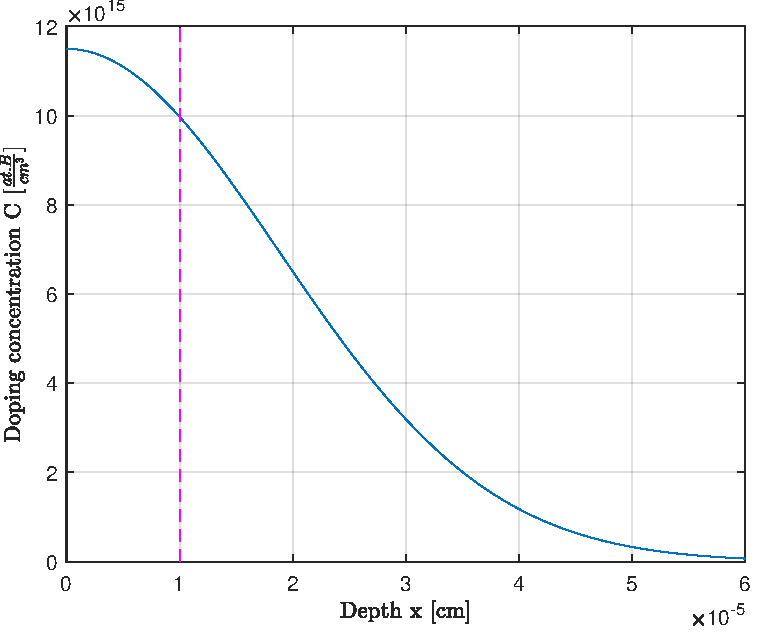
\includegraphics[width=100mm]{dopingadj1}
		\caption{Doping concentration for threshold adjustment}
		\label{dopingadj1}
	\end{figure}	
		\begin{table}
		\captionsetup{oneside,margin={2cm,0cm},justification = RaggedRight}
		\caption{Threshold adjustment, first attempt.}
		\centering
		\begin{tabular}[H]{|| c | c | c ||}
			\hline
			Parameter & Value & Measure Unit \\ [0.5ex] 
			\hline\hline
			$C_{ox}$ & 113 & $\frac{nF}{cm^2}$\\
			\hline
			$\Delta V_{TH}$ & 0.78 & $V$\\
			\hline
			$N_{ii}$ & $ 5.4\cdot 10^{11}$ & $\frac{at.B}{cm^2}$\\
			\hline			
			$\Delta r_p$ & 0.18 & $\mu m$\\
			\hline		
			$C_p$ & $1.15\cdot10^{16}$ & $\mu m$\\
			\hline		
			$C_j$ & $10^{16}$ & $\frac{at.B}{cm^3}$\\
			\hline			
			$x_j$ & 0.1 & $\mu m$\\
			\hline			
		\end{tabular}
		\label{adjparam}
	\end{table}
	\begin{table}
		\captionsetup{oneside,margin={2cm,0cm},justification = RaggedRight}
		\caption{Final threshold adjustment parameters.}
		\centering
		\begin{tabular}[H]{|| c | c | c ||}
			\hline
			Parameter & Value & Measure Unit \\ [0.5ex] 
			\hline\hline
			$N_{ii}$ & $ 5\cdot5.4\cdot 10^{11}$ & $\frac{at.B}{cm^2}$\\
			\hline			
			$\Delta r_p$ & 0.23 & $\mu m$\\
			\hline	
			$C_p$ & $5.005\cdot10^{16}$ & $\frac{at.B}{cm^3}$\\
			\hline		
			$C_j$ & $10^{16}$ & $\frac{at.B}{cm^3}$\\
			\hline			
			$x_j$ & 0.42 & $\mu m$\\
			\hline		
			$\int_{0}^{0.1}C(x)dx$ & $4.86\cdot10^{11}$ & $\frac{at.B}{cm^3}$\\
			\hline
			$V_{TH}$ & 1.03 & $V$\\
			\hline			
		\end{tabular}
		\label{adjparamfinal}
	\end{table}
	\begin{figure}
		\centering
		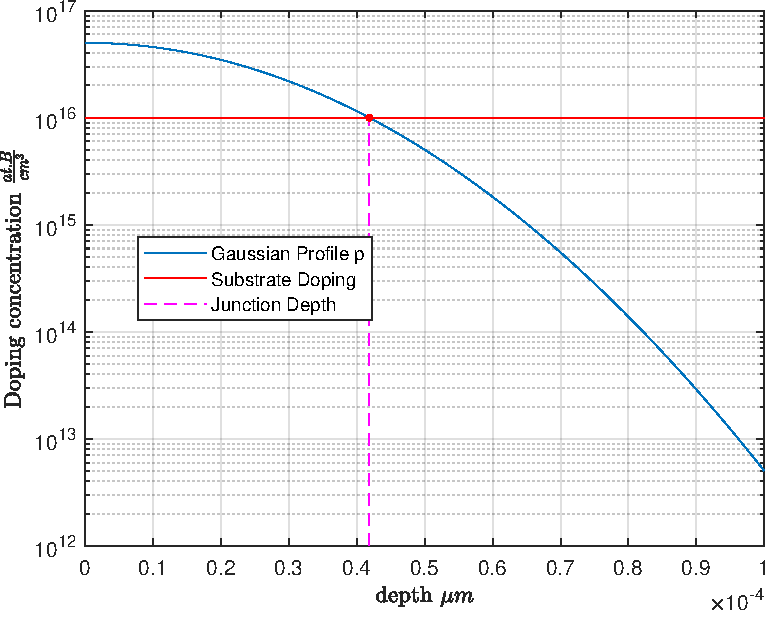
\includegraphics[width=100mm]{dopingadj2}
		\caption{Final doping concentration for threshold adjustment}
		\label{dopingadj2}
	\end{figure}
	\subsection{Equilibrium}
%	\subsection{Results}
		The previous simulations are done again, starting by the equilibrium condition one. In figure \ref*{equilibrium12} the results are presented, where the left part of the section is about the previous simulation and the right side is about the new one. Since these results are symmetric with respect to the midline, there is no loss of information due to the overlapping. In figure \ref*{equilibrium1} it can be seen that the depletion region in quite narrower, increasing the expected gate capacitance. In figure \ref*{equilibrium2} there is no significant change of behaviour in the substrate but in the corner of the space charge region. The orange region has more or less the same total current density, but it is more concentrated due to due different shape of the corner.
		\begin{figure}
			\centering
			\begin{subfigure}[b]{0.45\textwidth}
				\centering
				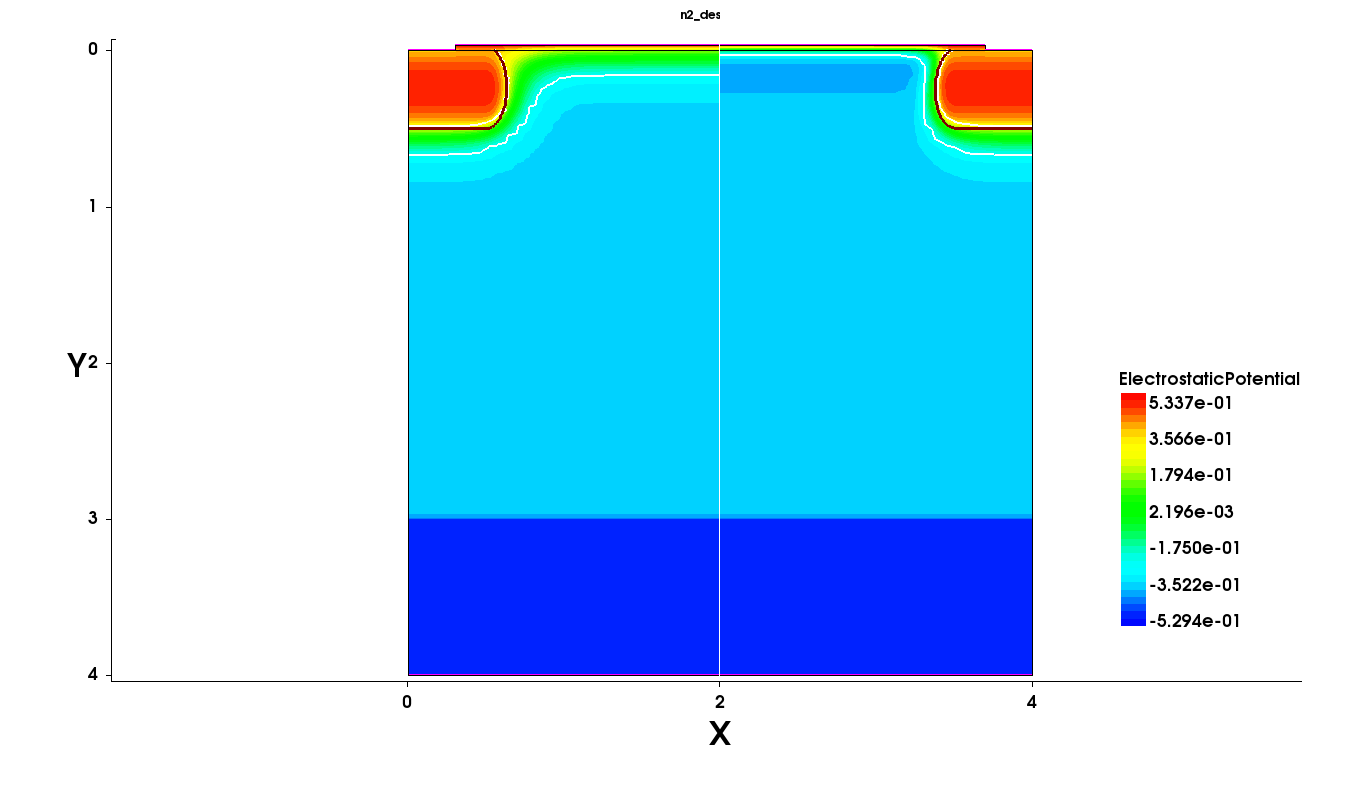
\includegraphics[width=\textwidth]{electrostatic_potential1122}
				\caption{Electrostatic Potential.}
				\label{equilibrium1}
			\end{subfigure}
			\hfill
			\begin{subfigure}[b]{0.45\textwidth}
				\centering
				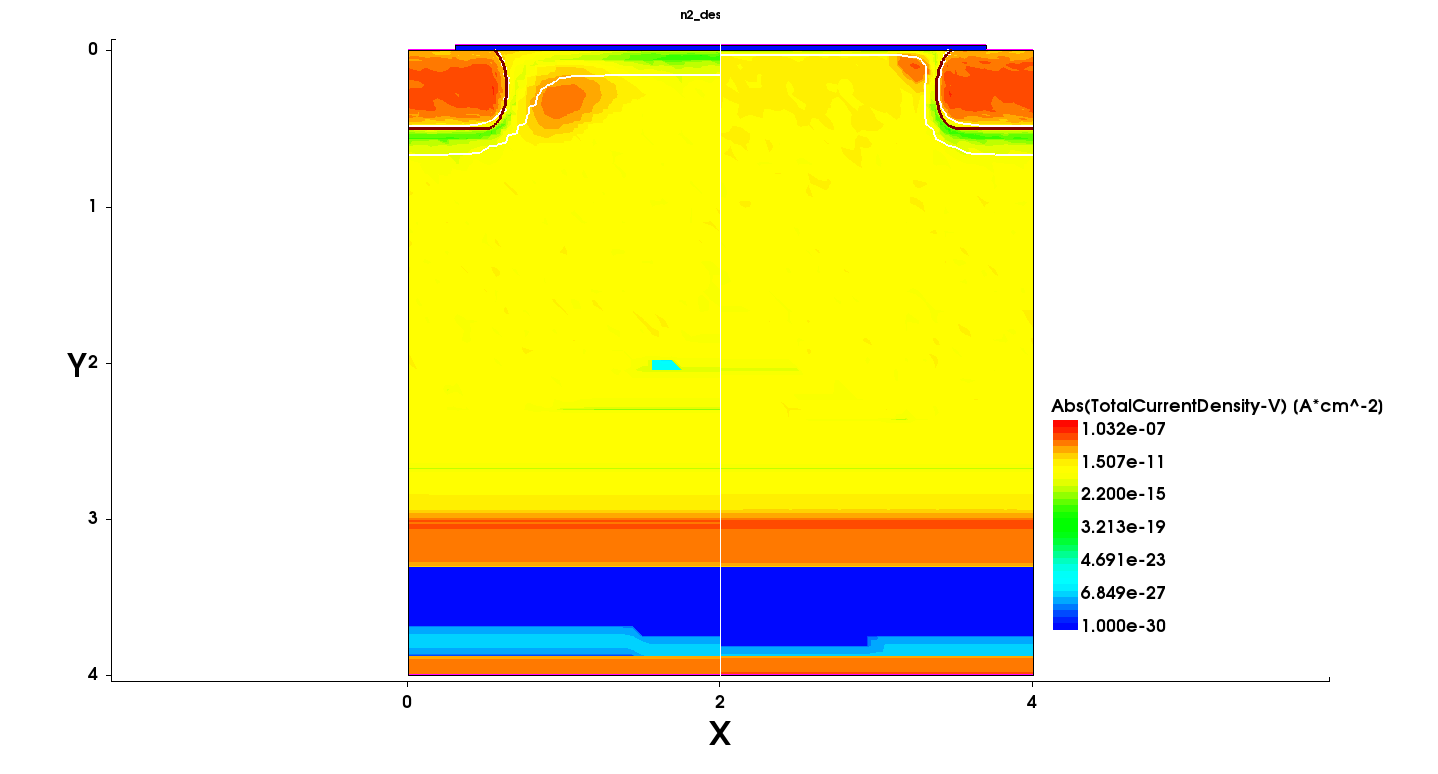
\includegraphics[width=\textwidth]{currents1122}
				\caption{Current density.}
				\label{equilibrium2}
			\end{subfigure}
			\caption{Simulation at equilibrium condition before and after threshold adjustment.}
			\label{equilibrium12}
		\end{figure}
		
	\subsection{Transfer Characteristic}
	The simulations about the transfer characteristic gives a parabola-shaped signal as expected (figure \ref*{parabola2}), and the identification procedure gives the values collected in table \ref*{identification_results2}
		\begin{figure}
			\centering
			\begin{subfigure}[b]{0.45\textwidth}
				\centering
				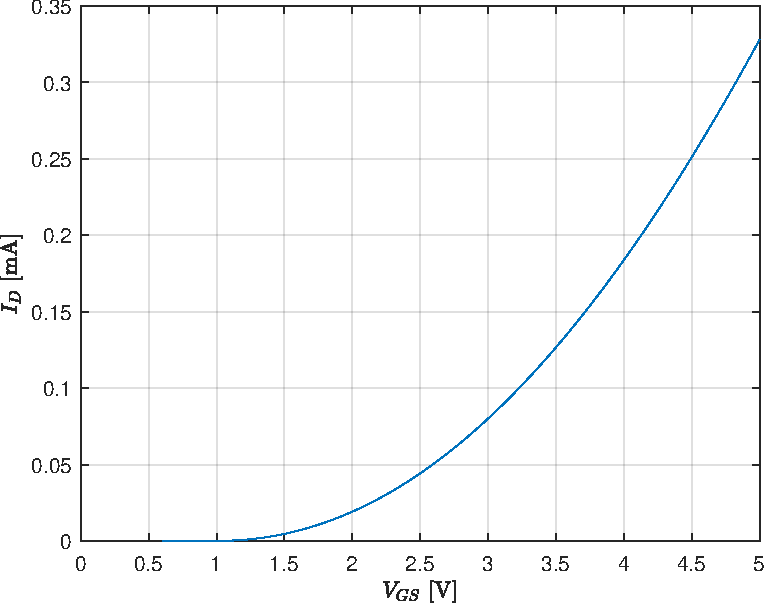
\includegraphics[width=\textwidth]{parabola2}
				\caption{Simulated transfer characteristic.}
				\label{parabola2}
			\end{subfigure}
			\hfill
			\begin{subfigure}[b]{0.45\textwidth}
				\centering
				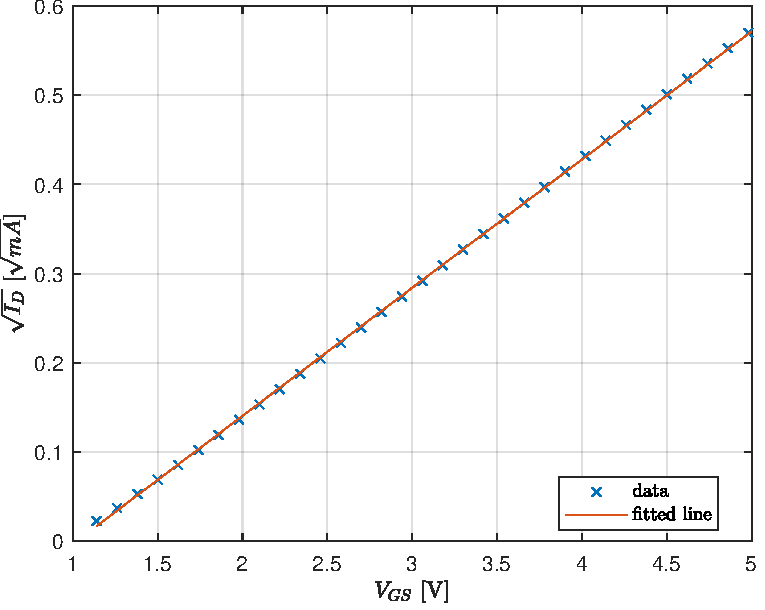
\includegraphics[width=\textwidth]{sqrt_fit2}
				\caption{Square root of drain current.}
				\label{sqrt_fit2}
			\end{subfigure}
			\caption{Identification of Threshold and Current Gain.}
			\label{identification2}
		\end{figure}
		\begin{table}
			\captionsetup{oneside,margin={2cm,0cm},justification = RaggedRight}
			\caption{Results of the identification}
			\centering
			\begin{tabular}[H]{|| c | c | c ||}
				\hline
				Parameter & Value & Measure Unit \\ [0.5ex] 
				\hline\hline
				$V_{TH}$ & 1.03 & $V$\\
				\hline
				$\beta$ & $4.13\cdot 10^{-2}$ & $\frac{mA}{V^2}$\\
				\hline			
			\end{tabular}
			\label{identification_results2}
		\end{table}
	\subsection{Small signal output resistance}
	At a first glance to the output characteristic, simulated and presented in figure \ref*{outputcurve2}, it can be seen that the slope of the tangent lines is generally lower than before. This behaviour results in a higher value of the small signal resistances, listed in table \ref*{resistances_adj}. This experiment confirms that the threshold value significantly affects the channel modulation length $\lambda$.
		\begin{figure}
			\centering
			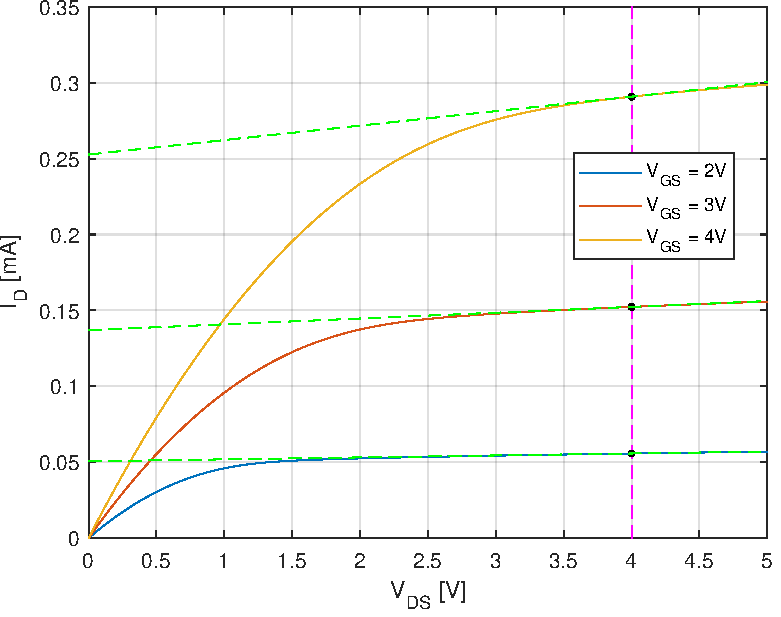
\includegraphics[width=100mm]{output_curves_adj}
			\caption{Output characteristic after threshold adjustment}
			\label{outputcurve2}
		\end{figure}
		\begin{table}
			\captionsetup{oneside,margin={2cm,0cm},justification = RaggedRight}
			\caption{Small signal output resistances after threshold adjustment}
			\centering
			\begin{tabular}{|| c | c | c | c ||}
				\hline
				Gate Bias & $[V]$ & Resistance & $[k\Omega]$ \\ [0.5ex] 
				\hline\hline
				$V_{GS2}$ & 2 & $R_{ss2}$& 777\\
				\hline
				$V_{GS3}$ & 3 & $R_{ss3}$& 261\\
				\hline
				$V_{GS4}$ & 4 & $R_{ss4}$& 105\\
				\hline			
			\end{tabular}
			\label{resistances_adj}
		\end{table}
	\subsection{Gate capacitance}
	As expected by the space charge width reduction, the overall gate capacitance increased. The only parts that remain unchanged despite the threshold adjustment are the minimum and maximum values. The maximum is equal to $C_{ox}$ because in both cases the oxide geometry and properties is same same. The minimum depends on $C_{min}$ (equation \ref*{cmin}), which is constant as long as $V_{GS}$ is higher than the threshold.  
		\begin{figure}
			\centering
			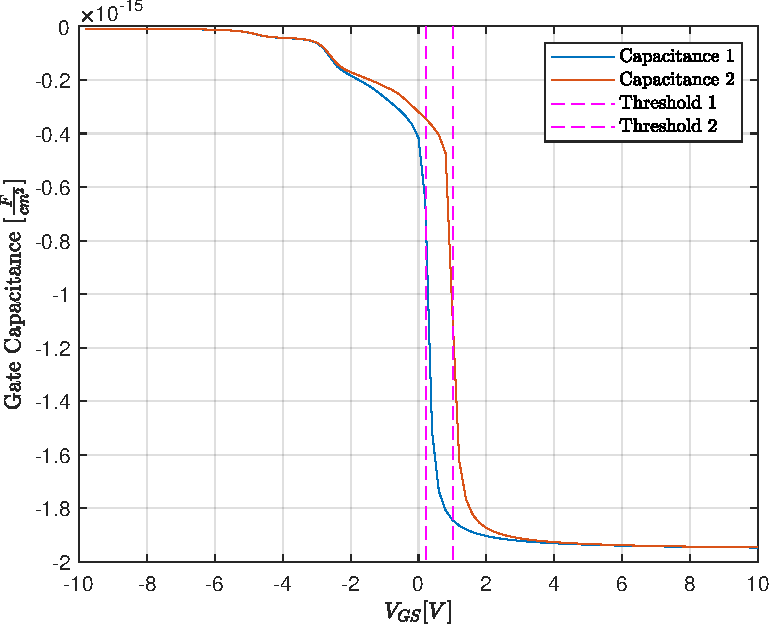
\includegraphics[width=100mm]{capacitance12}
			\caption{Gate capacitance before and after threshold adjustment.}
			\label{capacitance12}
		\end{figure}
	\newpage
	\hypersetup{linkcolor = black}
	\listoffigures
	\listoftables
\end{document}